\documentclass{standalone}
\usepackage{tikz}
\usepackage{ctex,siunitx}
\setCJKmainfont{Noto Serif CJK SC}
\usepackage{tkz-euclide}
\usepackage{amsmath}
\usetikzlibrary{patterns, calc}
\usetikzlibrary {decorations.pathmorphing, decorations.pathreplacing, decorations.shapes,}

\begin{document}
\small
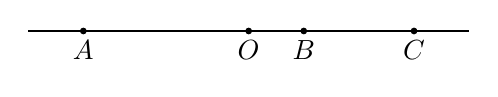
\begin{tikzpicture}[>=stealth,scale=0.7]
  \tkzSetUpPoint[fill=black]
  % \useasboundingbox(-1,-0.75)rectangle(3.7,1.4);
  \draw (0,0)--(8,0);
  \tkzDefPoints{1/0/A,5/0/B,7/0/C, 4/0/O}
  \tkzDrawPoints(A,B,C,O)
  \tkzLabelPoints[below](A,B,C,O)	
\end{tikzpicture}
\end{document}